\begin{figure}[t]
  \center
  \def\layersep{1.8cm}
  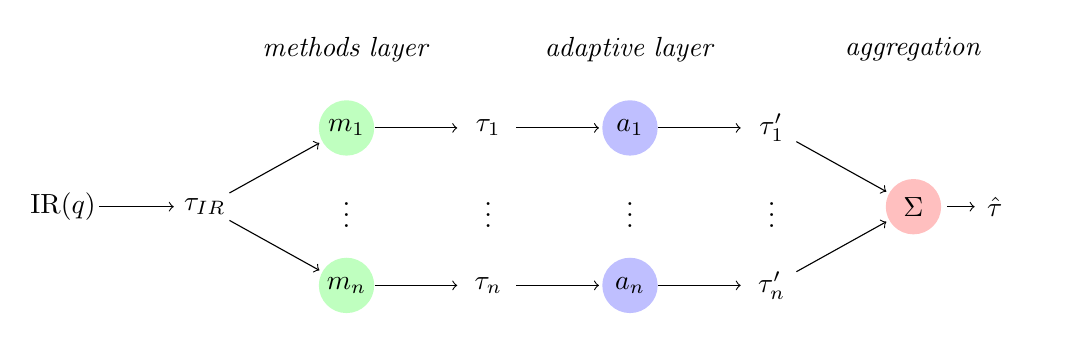
\begin{tikzpicture}[shorten >=1pt,->,draw=black, node distance=\layersep]

    \tikzstyle{every pin edge}=[<-,shorten <=2pt]
    \tikzstyle{node}=[circle,fill=black!25,minimum size=20pt,inner sep=0pt]
    \tikzstyle{input node}=[node, fill=green!25];
    \tikzstyle{output node}=[node, fill=red!25];
    \tikzstyle{hidden node}=[node, fill=blue!25];
    \tikzstyle{annot} = [text width=10em, text centered]
    \tikzstyle{txt}=[node,fill=white];
    

    \node[txt] (IR) at (0,-2) {$\mathrm{IR}(q)$};
    \node[txt] (UI) at (\layersep,-2) {$\tau_{IR}$};  

    \node[input node] (I-1) at (\layersep*2,-1) {$m_1$};
    \node[txt]        (I-D) at (\layersep*2,-2) {$\vdots$};
    \node[input node] (I-N) at (\layersep*2,-3) {$m_n$};
    
    \node[txt] (P-1) at (\layersep*3, -1) {$\tau_1$};
    \node[txt] (P-D) at (\layersep*3, -2) {$\vdots$};
    \node[txt] (P-N) at (\layersep*3, -3) {$\tau_n$};

    \node[hidden node] (H-1) at (\layersep*4, -1) {$a_1$};    
    \node[txt]         (H-D) at (\layersep*4, -2) {$\vdots$};    
    \node[hidden node] (H-N) at (\layersep*4, -3) {$a_n$};    

    \node[txt] (R-1) at (\layersep*5, -1) {$\tau_1^\prime$};
    \node[txt] (R-D) at (\layersep*5, -2) {$\vdots$};
    \node[txt] (R-N) at (\layersep*5, -3) {$\tau_n^\prime$};
    
    % hidden helper node
    \node[txt] (HH)  at (\layersep*6,-1) {};
    % Draw the output layer node
    \node[output node,pin={[pin edge={->}]right:$\hat{\tau}$}] at (\layersep*6,-2) (O) {$\Sigma$};
    
    \path (IR) edge (UI);
       
    \path (UI) edge (I-1);
    \path (UI) edge (I-N);

    \path (I-1) edge (P-1);
    \path (I-N) edge (P-N);

    \path (P-1) edge (H-1);
    \path (P-N) edge (H-N);

    \path (H-1) edge (R-1);
    \path (H-N) edge (R-N);

    \path (R-1) edge (O);
    \path (R-N) edge (O);

    % Annotate the layers
    \node[annot,above of=I-1, node distance=1cm] {\emph{methods layer}};
    \node[annot,above of=H-1, node distance=1cm] {\emph{adaptive layer}};
    \node[annot,above of=HH,  node distance=1cm] {\emph{aggregation}};
  \end{tikzpicture}

  \vspace{1em}
  \caption[Example of Adaptive Rank Aggregation]{
    Example of Adaptive Rank Aggregation: 
    An IR method returns a results list of possibly related items, each with a ranking score.
    The methods layer estimates ratings for each item in the results list.
    The adaptive layer predicts how accurate ach of these ratings are likely to be.
    Finally, the ranking scores, ratings and accuracy estimations are combined
    into one result list, $\hat{\tau}$.
  }
  \label{fig:adaptiverank}
\end{figure}
